\chapter*{Úvod}
\phantomsection
\addcontentsline{toc}{chapter}{Úvod}


%Tato práce se věnuje oblast i \zk{zkDSP} (\zkratkatext{zkDSP}), zejména jevům, které nastanou při nedodržení Nyquistovy podmínky pro \zkratka{symfvz}.%
%\footnote{Tato věta je pouze ukázkou použití příkazů pro sazbu zkratek.}

%\begin{figure}[!h]
%	\begin{center}
%		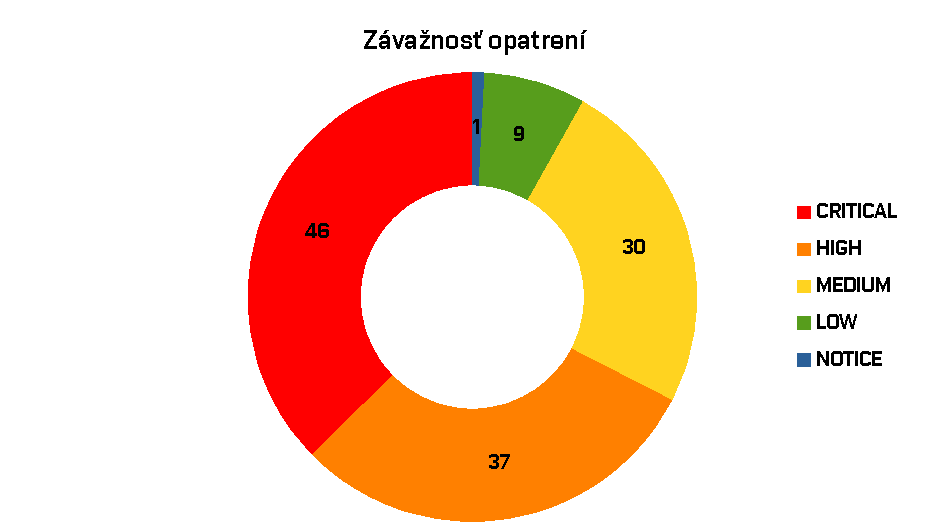
\includegraphics[scale=0.5]{obrazky/zavaznosti_graf.pdf}
%	\end{center}
%	\caption[graf_zavaznost]{Závažnosť opatrení}
%
%\end{figure}

Kybernetická bezpečnosť je bezpochyby jednou z hlavných tém 21. storočia. Útoky na infraštruktúru a systémy naberajú nielen na frekvencii, ale čo je ešte horšie na sofistikovanosti. Napriek častému zdôrazňovaniu odborníkov o kladenie čoraz väčšieho dôrazu na bezpečnosť pri návrhu, implementácii a nasadeniu, sa stále stretávame s fatálnymi dôsledkami, ktoré boli spôsobené nedostatočným venovaním pozornosti bezpečnosti. 

Problém nedostatočného zabezpečenia nie je ani tak nevedomosť základných bezpečnostných praktík administrátorov alebo programátorov, ale potreba rýchleho nasadenia systému a infraštruktúry s odložením implementácie bezpečnostných praktík na neskôr. Tieto problémy vznikajú aj pri dodatočnej implementácií nových modulov a pridaní novej infraštruktúry, kedy sa nemení celok, ale pridanie jednej časti môže výrazne ovplyvniť a zmeniť stav bezpečnosti celého systému. Z tohto dôvodu je priam žiadúce disponovať nejakým procesom alebo nástrojom na dodatočné zistenie nedostatkov a ich následnú elimináciu. Veľmi silnou motiváciou by malo byť aj to, že dôsledkom bezpečnostných nedostatkov sú globálne miliardové škody a straty reputácií firiem. 

Jednou z hlavných častí infraštruktúry, kde dochádza k významným bezpečnostným incidentom je počítačová sieť, bez ktorej by dnes informačné technológie nevedeli fungovať. Preto sa táto práca bude zaoberať práve ňou, keďže je vstupnou bránou do systémov a jej vyradením alebo zneužitím prichádzajú organizácie o finančné prostriedky, citlivé dáta a dôveru užívateľov.

Výsledkom tejto práce bude aplikácia overujúca nastavenia sieťových zariadení prevažne v lokálnej sieti, ktorá umožňuje zjednať nápravu na základe nájdených nedostatkov. Výhodou oproti existujúcim riešeniam bude otvorenosť kódu a modularita, ktorá umožní rozšírenie aplikácie na sieťové zariadenia rôznych výrobcov. Dôležitým výstupom bude taktiež zoznam bezpečnostných a prevádzkových odporučaní vychádzajúcich z rôznych štandardov a odporučaní, ktoré môžu byť v budúcnosti použité ďalšími užívateľmi aplikácie pri zostavovaní modulov pre zariadenia rôznych výrobcov. Jednou z kľúčových vlastností je bezplatnosť, keďže podľa zistení takmer polovica útokov smeruje na malé firmy, ktoré bezpečnosť často neriešia z finančnej náročnosti programov na detekciu bezpečnostných nedostatkov.    
